\documentclass[12pt]{article}
\usepackage[margin=1 in]{geometry}
\usepackage{graphicx}
\usepackage{float} % For [H] figure placement
\usepackage{booktabs} % For professional tables
\usepackage{siunitx} % For SI units
\usepackage{amsmath}
\usepackage{amssymb}
\usepackage{pgfplots} % For plotting
\pgfplotsset{compat=1.18}
\usepackage{fancyhdr} 
\usepackage{hyperref} 
\usepackage{circuitikz} % For drawing circuits
\usepackage{subcaption} 

\hypersetup{
    colorlinks=false, 
    hidelinks        
}
% Set paragraph formatting
\setlength{\parindent}{0in}
\setlength{\parskip}{\baselineskip}

% --- DOCUMENT INFORMATION ---
\title{Lab 10: BJT Common-Emitter Amplifier}
\author{Sean Balbale}
\date{November 30, 2025}

% --- BEGIN DOCUMENT ---
\begin{document}

% --- COVER SHEET ---
\begin{titlepage}
  \begin{center}
    \vspace*{1in}

    \Huge
    \textbf{Lab 10}

    \LARGE
    \vspace{0.5cm}
    BJT Common-Emitter Amplifier

    \vspace{3in}

    \textbf{Student Name:} Sean Balbale
    \\ \textbf{Instructor:} Debora Fixel
    \\ \textbf{Course:} ENGR 305
    \\ \textbf{Date:} November 30, 2025

    \vfill
  \end{center}
\end{titlepage}

\newpage

% --- OBJECTIVE ---
\section{Objective}
The objective of this laboratory exercise is to design, simulate, and characterize a BJT Common-Emitter (CE) amplifier. The specific goals are:
\begin{itemize}
  \item To design a CE amplifier with a specific quiescent current ($I_C = \SI{1}{mA}$) and a target voltage gain of $|A_v| = 200$ V/V.
  \item To perform a SPICE simulation to verify the DC operating point and AC small-signal performance.
  \item To build the circuit and measure the experimental gain, input/output impedances, and signal limits (clipping).
  \item To compare theoretical calculations, simulation results, and experimental measurements.
\end{itemize}

% --- THEORY ---
\section{Theory}
The Common-Emitter amplifier is a widely used configuration offering high voltage gain. In this experiment, a dual-supply topology ($V_{CC} = +15V$, $V_{EE} = -15V$) is used with an NPN transistor (2N3904).

\paragraph{DC Analysis}
The DC operating point (Q-point) determines the amplifier's region of operation. For linear amplification, the BJT must be in the active mode ($V_{BE} \approx 0.7V$ and $V_{CE} > 0.2V$).
The DC emitter current is determined by the emitter resistor $R_E$:
$$
I_E \approx \frac{V_B - V_{BE} - V_{EE}}{R_E}
$$
Assuming the base is at DC ground ($V_B \approx 0V$) and $V_{BE} \approx 0.7V$, $R_E$ sets the bias current. The collector current is $I_C \approx I_E$.

\paragraph{AC Small-Signal Analysis}
The voltage gain $A_v$ of a bypassed CE amplifier (where the emitter resistor is bypassed by a capacitor $C_E$ to ground) is given by:
$$
A_v = -g_m (R_C \parallel R_L)
$$
where $g_m$ is the transconductance of the BJT:
$$
g_m = \frac{I_C}{V_T} \approx \frac{I_C}{\SI{26}{mV}}
$$
The negative sign indicates a $180^{\circ}$ phase shift.
The output resistance $R_o$ of the amplifier (looking into the collector) is dominated by the collector resistor $R_C$, assuming the transistor's Early resistance $r_o$ is large ($r_o \gg R_C$).
$$
R_o \approx R_C
$$

% --- EXPERIMENTAL METHOD ---
\section{Experimental Method and Design}

\subsection{Design Procedure}
The circuit was designed to meet the following specifications:
\begin{itemize}
    \item $V_{CC} = +15V$, $V_{EE} = -15V$.
    \item Load Resistance $R_L = \SI{10}{k\Omega}$.
    \item Quiescent Current $I_C = \SI{1}{mA}$.
    \item Magnitude of Voltage Gain $|A_v| = 200$.
\end{itemize}

\textbf{1. Calculating $R_E$:}
To achieve $I_C \approx I_E = \SI{1}{mA}$ with the base at ground:
$$ R_E = \frac{0V - 0.7V - (-15V)}{\SI{1}{mA}} = \frac{14.3V}{\SI{1}{mA}} = \SI{14.3}{k\Omega} $$
(Standard value chosen: $14.3 \text{ k}\Omega$ or series combination).

\textbf{2. Calculating $R_C$:}
The transconductance is $g_m = \frac{1\text{ mA}}{26\text{ mV}} = \SI{38.46}{mS}$.
Using the gain equation $|A_v| = g_m (R_C \parallel R_L)$:
$$ 200 = (38.46 \times 10^{-3}) \left( \frac{R_C \cdot 10k}{R_C + 10k} \right) $$
Solving for the equivalent AC load: $R_{AC} = \frac{200}{0.03846} = \SI{5.2}{k\Omega}$.
$$ \frac{1}{R_C} = \frac{1}{5.2k} - \frac{1}{10k} \implies R_C \approx \SI{10.83}{k\Omega} $$
(Standard value chosen: $10.8 \text{ k}\Omega$).

\subsection{Simulation}
The designed circuit was simulated in LTspice using the 2N3904 model. 

\begin{figure}[H]
    \centering
    \includegraphics[width=0.8\textwidth]{Screenshot 2025-11-30 163957.png}
    \caption{LTSpice schematic and simulation results.}
    \label{fig:ltspice}
\end{figure}

\subsection{Experimental Setup}
The circuit was constructed on a breadboard as shown in Figure \ref{fig:breadboard}. 
\begin{figure}[H]
    \centering
    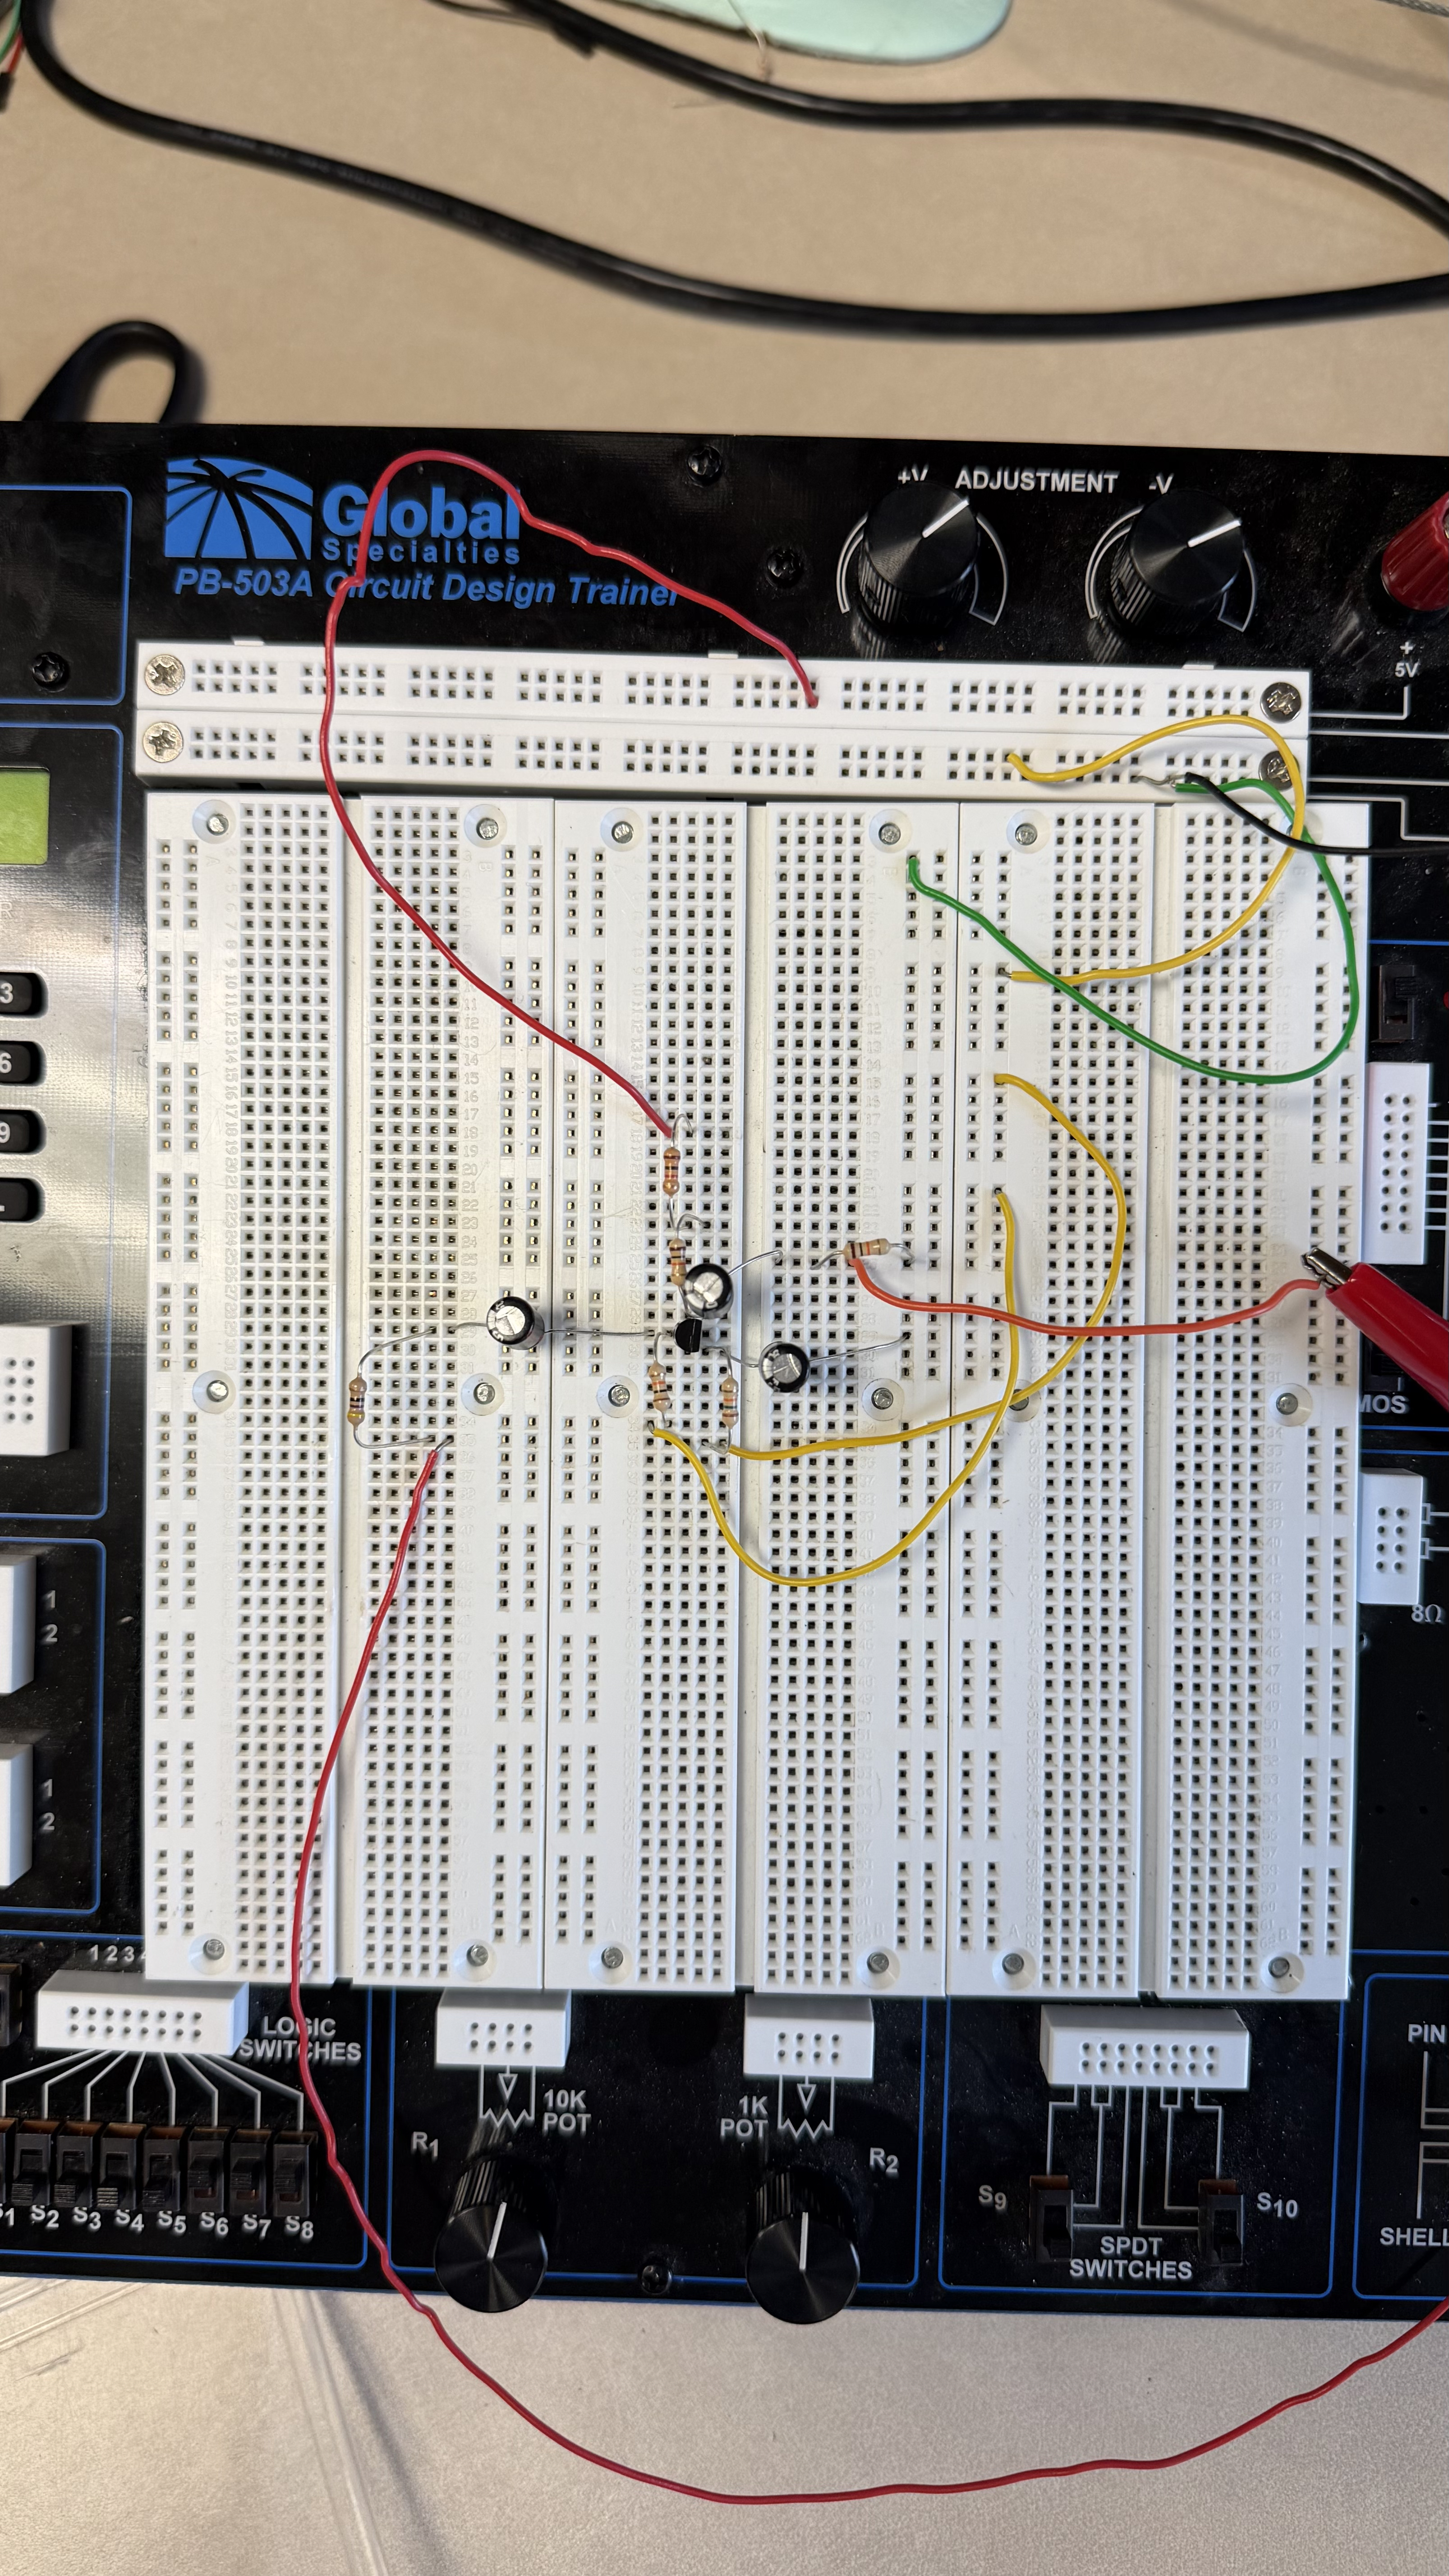
\includegraphics[width=0.6\textwidth]{IMG_0883.png}
    \caption{The assembled Common-Emitter amplifier on the breadboard.}
    \label{fig:breadboard}
\end{figure}

The measurements were performed as follows:
\begin{itemize}
    \item \textbf{Gain Measurement:} $v_{in}$ was set to $\approx 24 \text{ mV}_{\text{pk-pk}}$ at $10 \text{ kHz}$. $v_{out}$ was measured across $R_L = 10k\Omega$.
    \item \textbf{Output Resistance ($R_o$):} The output was measured first with an open load ($R_L \approx \SI{1}{M\Omega}$), and then with a specific load resistor ($R_L = \SI{9.1}{k\Omega}$) to observe the voltage drop.
\end{itemize}

% --- RESULTS AND DISCUSSION ---
\section{Results and Discussion}

\subsection{DC Operating Point}
The DC voltages and currents were calculated, simulated, and measured. The results are summarized below.

\begin{table}[H]
  \centering
  \caption{DC Operating Point Comparison}
  \label{tab:dc_compare}
  \sisetup{round-mode=places,round-precision=3}
  \begin{tabular}{lccc}
    \toprule
    \textbf{Parameter} & \textbf{Calculated} & \textbf{Simulated} & \textbf{Measured} \\
    \midrule
    $V_C$ (Collector) & \SI{4.17}{\volt} & \SI{4.01}{\volt} & \SI{4.17}{\volt} \\
    $V_B$ (Base) & \SI{0}{\volt} & \SI{-0.033}{\volt} & \SI{-0.017}{\volt} \\
    $V_E$ (Emitter) & \SI{-0.7}{\volt} & \SI{-0.687}{\volt} & \SI{-0.718}{\volt} \\
    $I_C$ & \SI{1.0}{\milli\ampere} & \SI{1.01}{\milli\ampere} & \SI{1.01}{\milli\ampere} \\
    \bottomrule
  \end{tabular}
\end{table}

\textbf{Analysis:} The DC results show exceptional agreement. The measured Collector Voltage ($V_C = \SI{4.17}{V}$) matches the calculation exactly. The Base Voltage ($V_B$) is slightly negative ($\SI{-17}{mV}$) due to the small voltage drop across the base resistor caused by the base current $I_B$.

\subsection{AC Performance and Gain}

\begin{figure}[H]
    \centering
    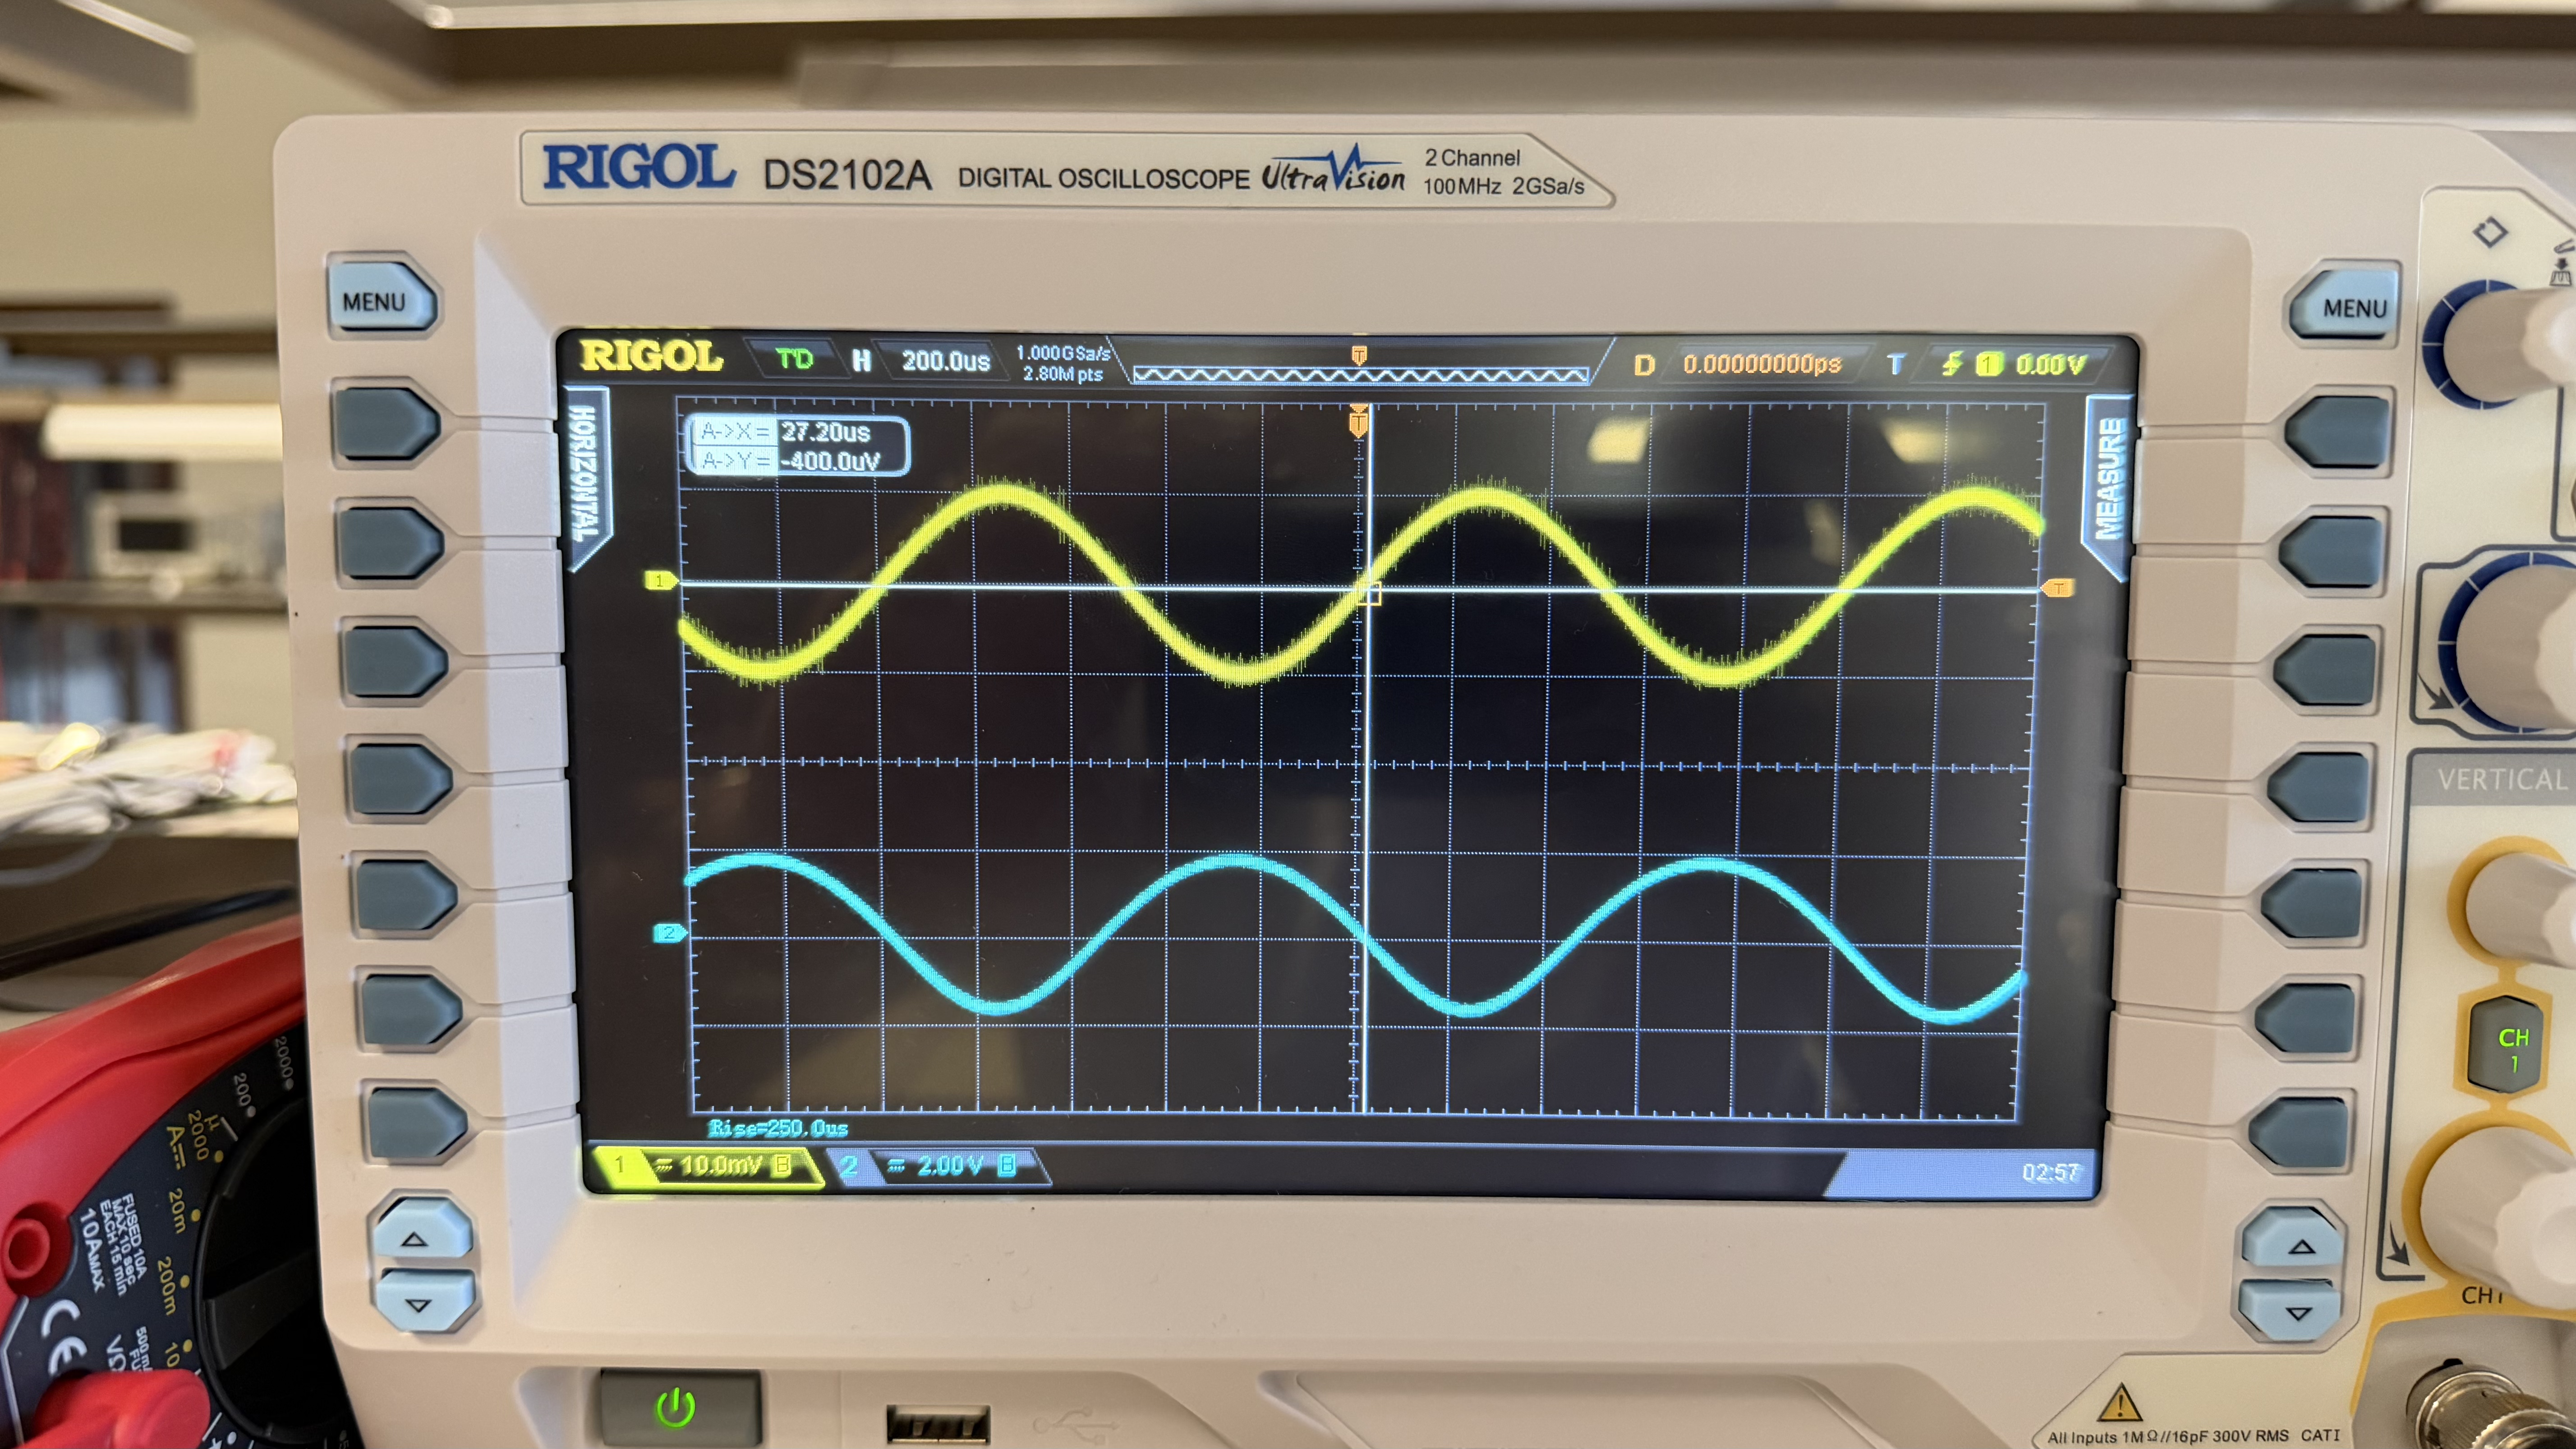
\includegraphics[width=0.7\textwidth]{IMG_0890.png}
    \caption{Oscilloscope measurement of Gain with $R_L = \SI{10}{k\Omega}$. Input (Yellow) and Output (Blue).}
    \label{fig:gain_meas}
\end{figure}

\begin{table}[H]
  \centering
  \caption{AC Performance Comparison}
  \label{tab:ac_compare}
  \begin{tabular}{lccc}
    \toprule
    \textbf{Parameter} & \textbf{Design Goal} & \textbf{Simulated} & \textbf{Measured} \\
    \midrule
    Input ($v_{in}$) & -- & $10 \text{ mV}_{\text{pp}}$ & $24 \text{ mV}_{\text{pp}}$ \\
    Output ($v_{out}$) & -- & $1.90 \text{ V}_{\text{pp}}$ & $4.88 \text{ V}_{\text{pp}}$ \\
    \textbf{Gain ($A_v$)} & \textbf{-200 V/V} & \textbf{-190 V/V} & \textbf{-203.3 V/V} \\
    \bottomrule
  \end{tabular}
\end{table}

\textbf{Analysis:} 
As seen in Figure \ref{fig:gain_meas}, the measured gain was:
$$ A_{v(measured)} = \frac{v_{out}}{v_{in}} = \frac{4.88\text{ V}}{0.024\text{ V}} \approx 203.3 \text{ V/V} $$
This is remarkably close to the design goal of 200 (an error of only 1.6\%).

\subsection{Output Resistance ($R_o$)}
The output resistance was determined experimentally by comparing the "Open Load" output voltage to the "Loaded" output voltage.

\begin{figure}[H]
    \centering
    \begin{subfigure}{0.48\textwidth}
        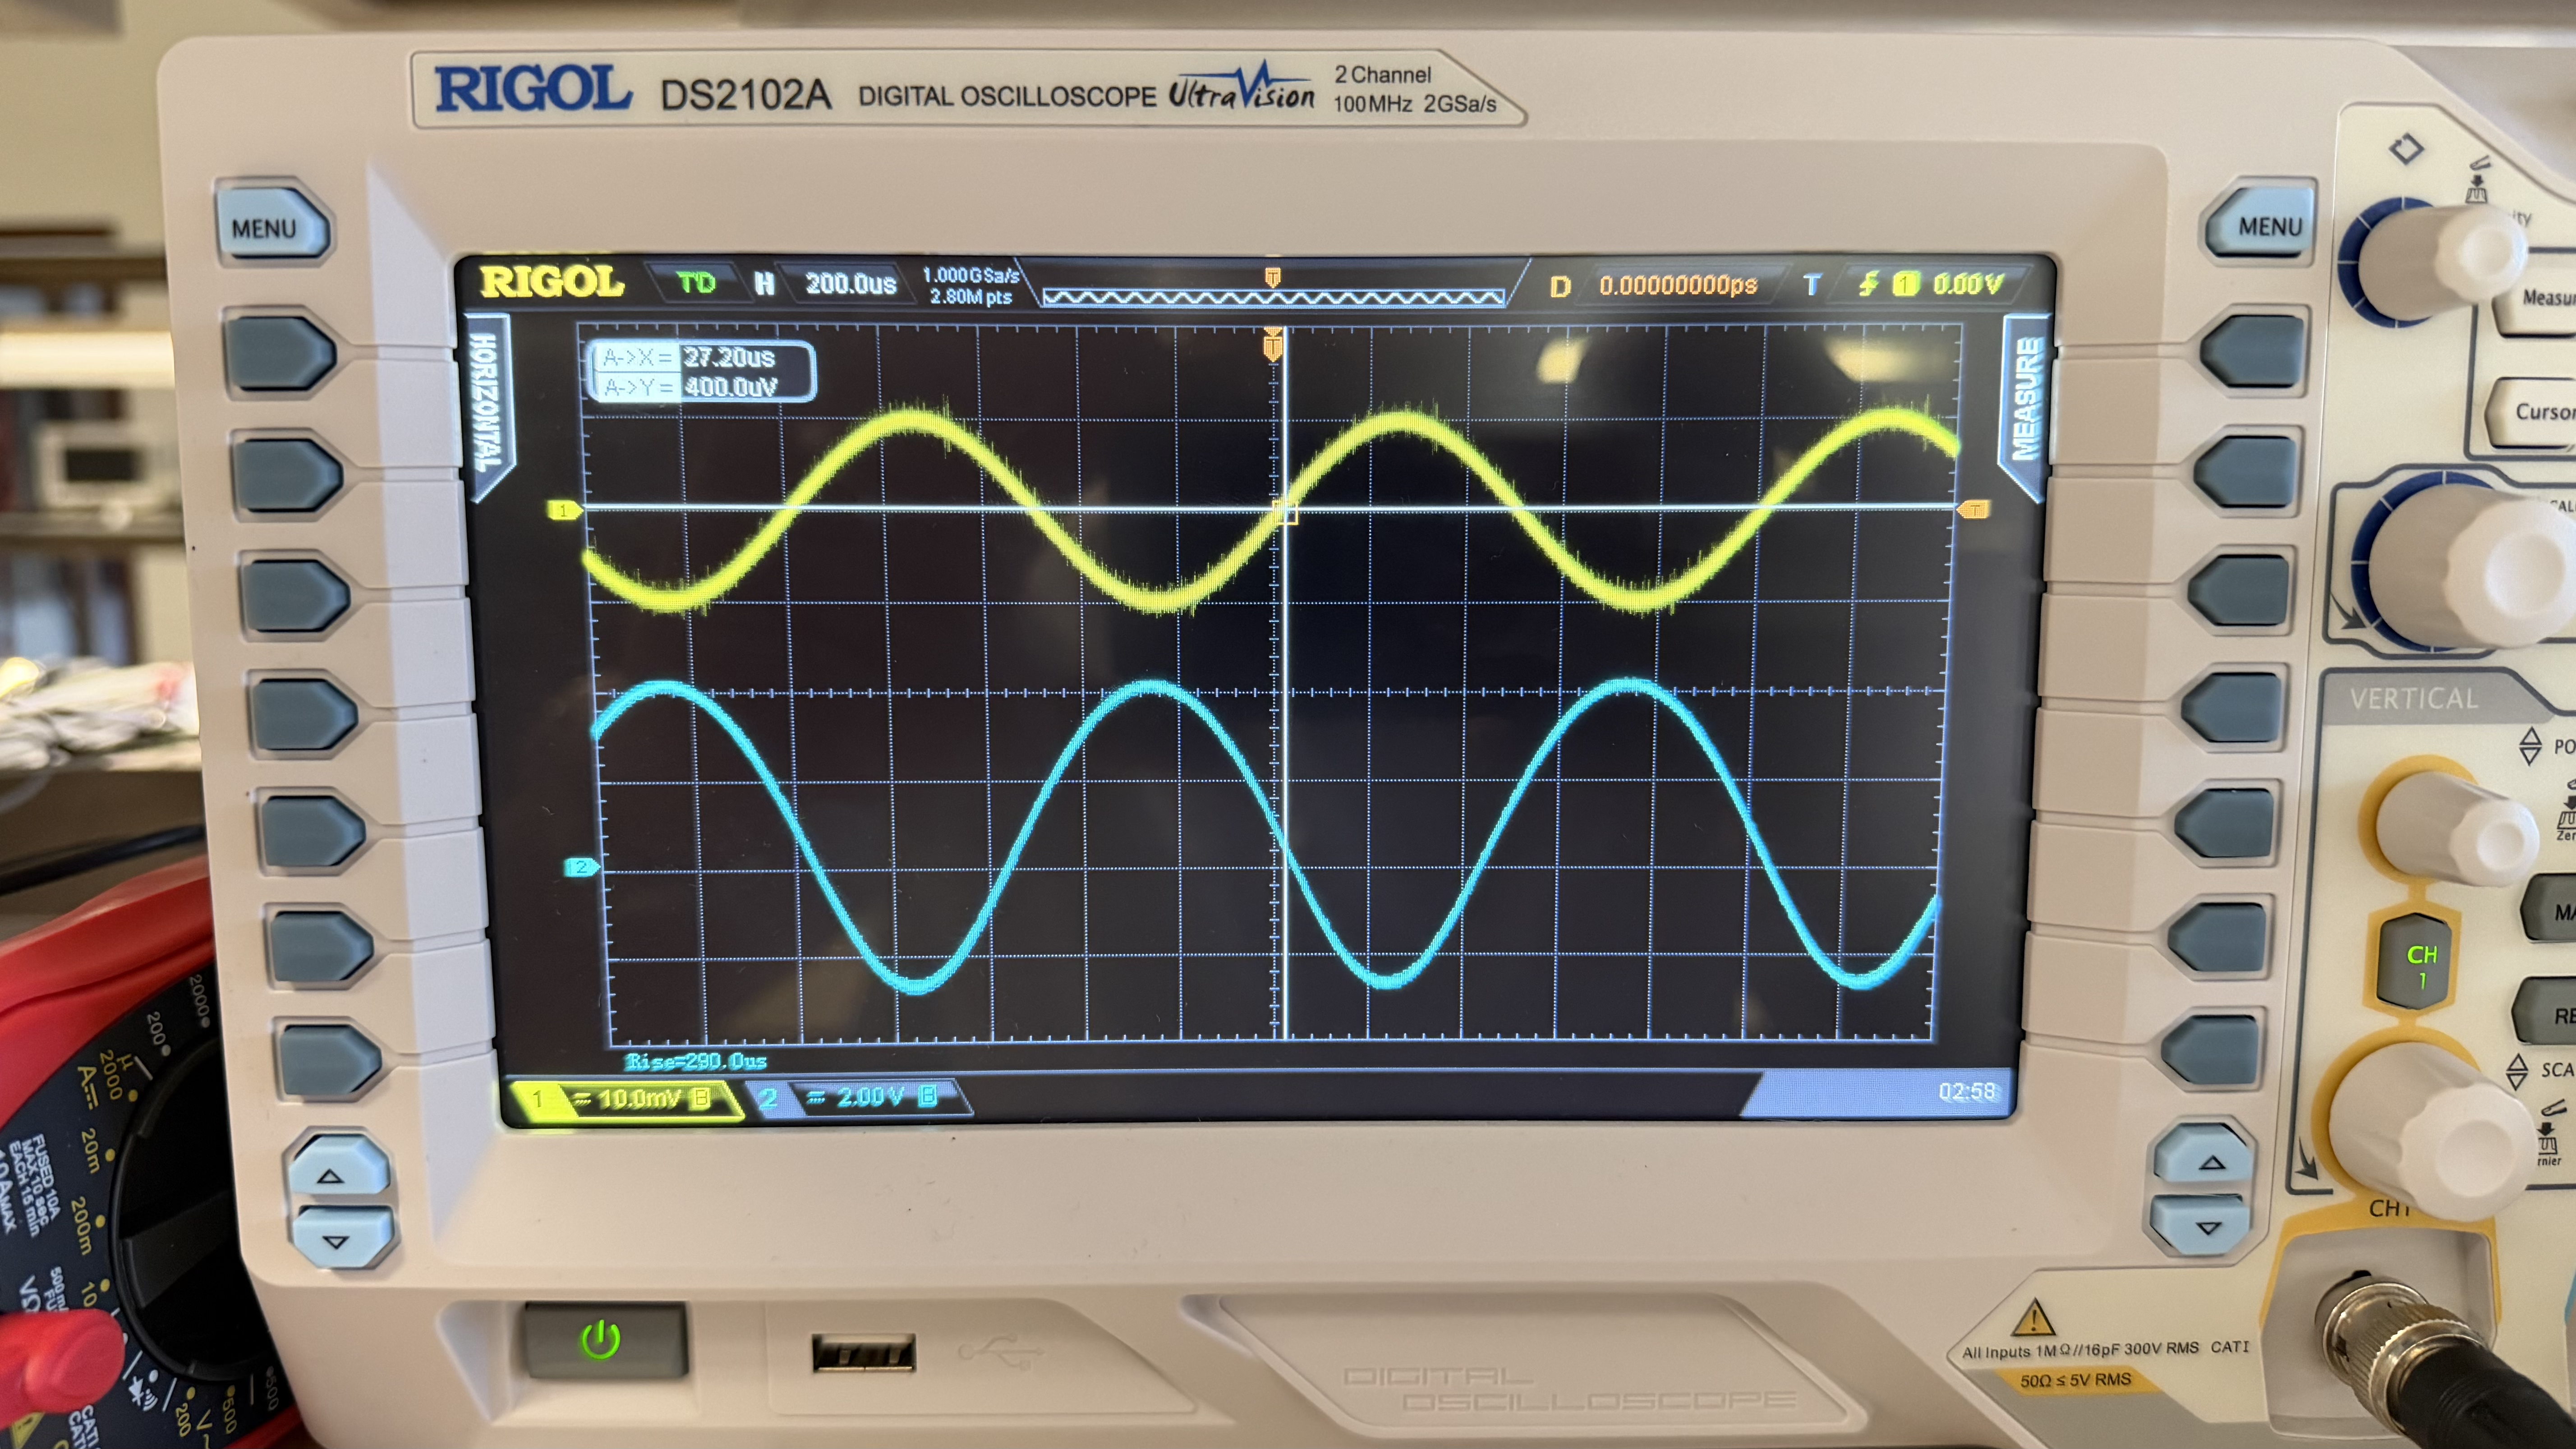
\includegraphics[width=\textwidth]{IMG_0892.png}
        \caption{Open Load ($R_L = \SI{1}{M\Omega}$): High Output Amplitude.}
        \label{fig:open_load}
    \end{subfigure}
    \hfill
    \begin{subfigure}{0.48\textwidth}
        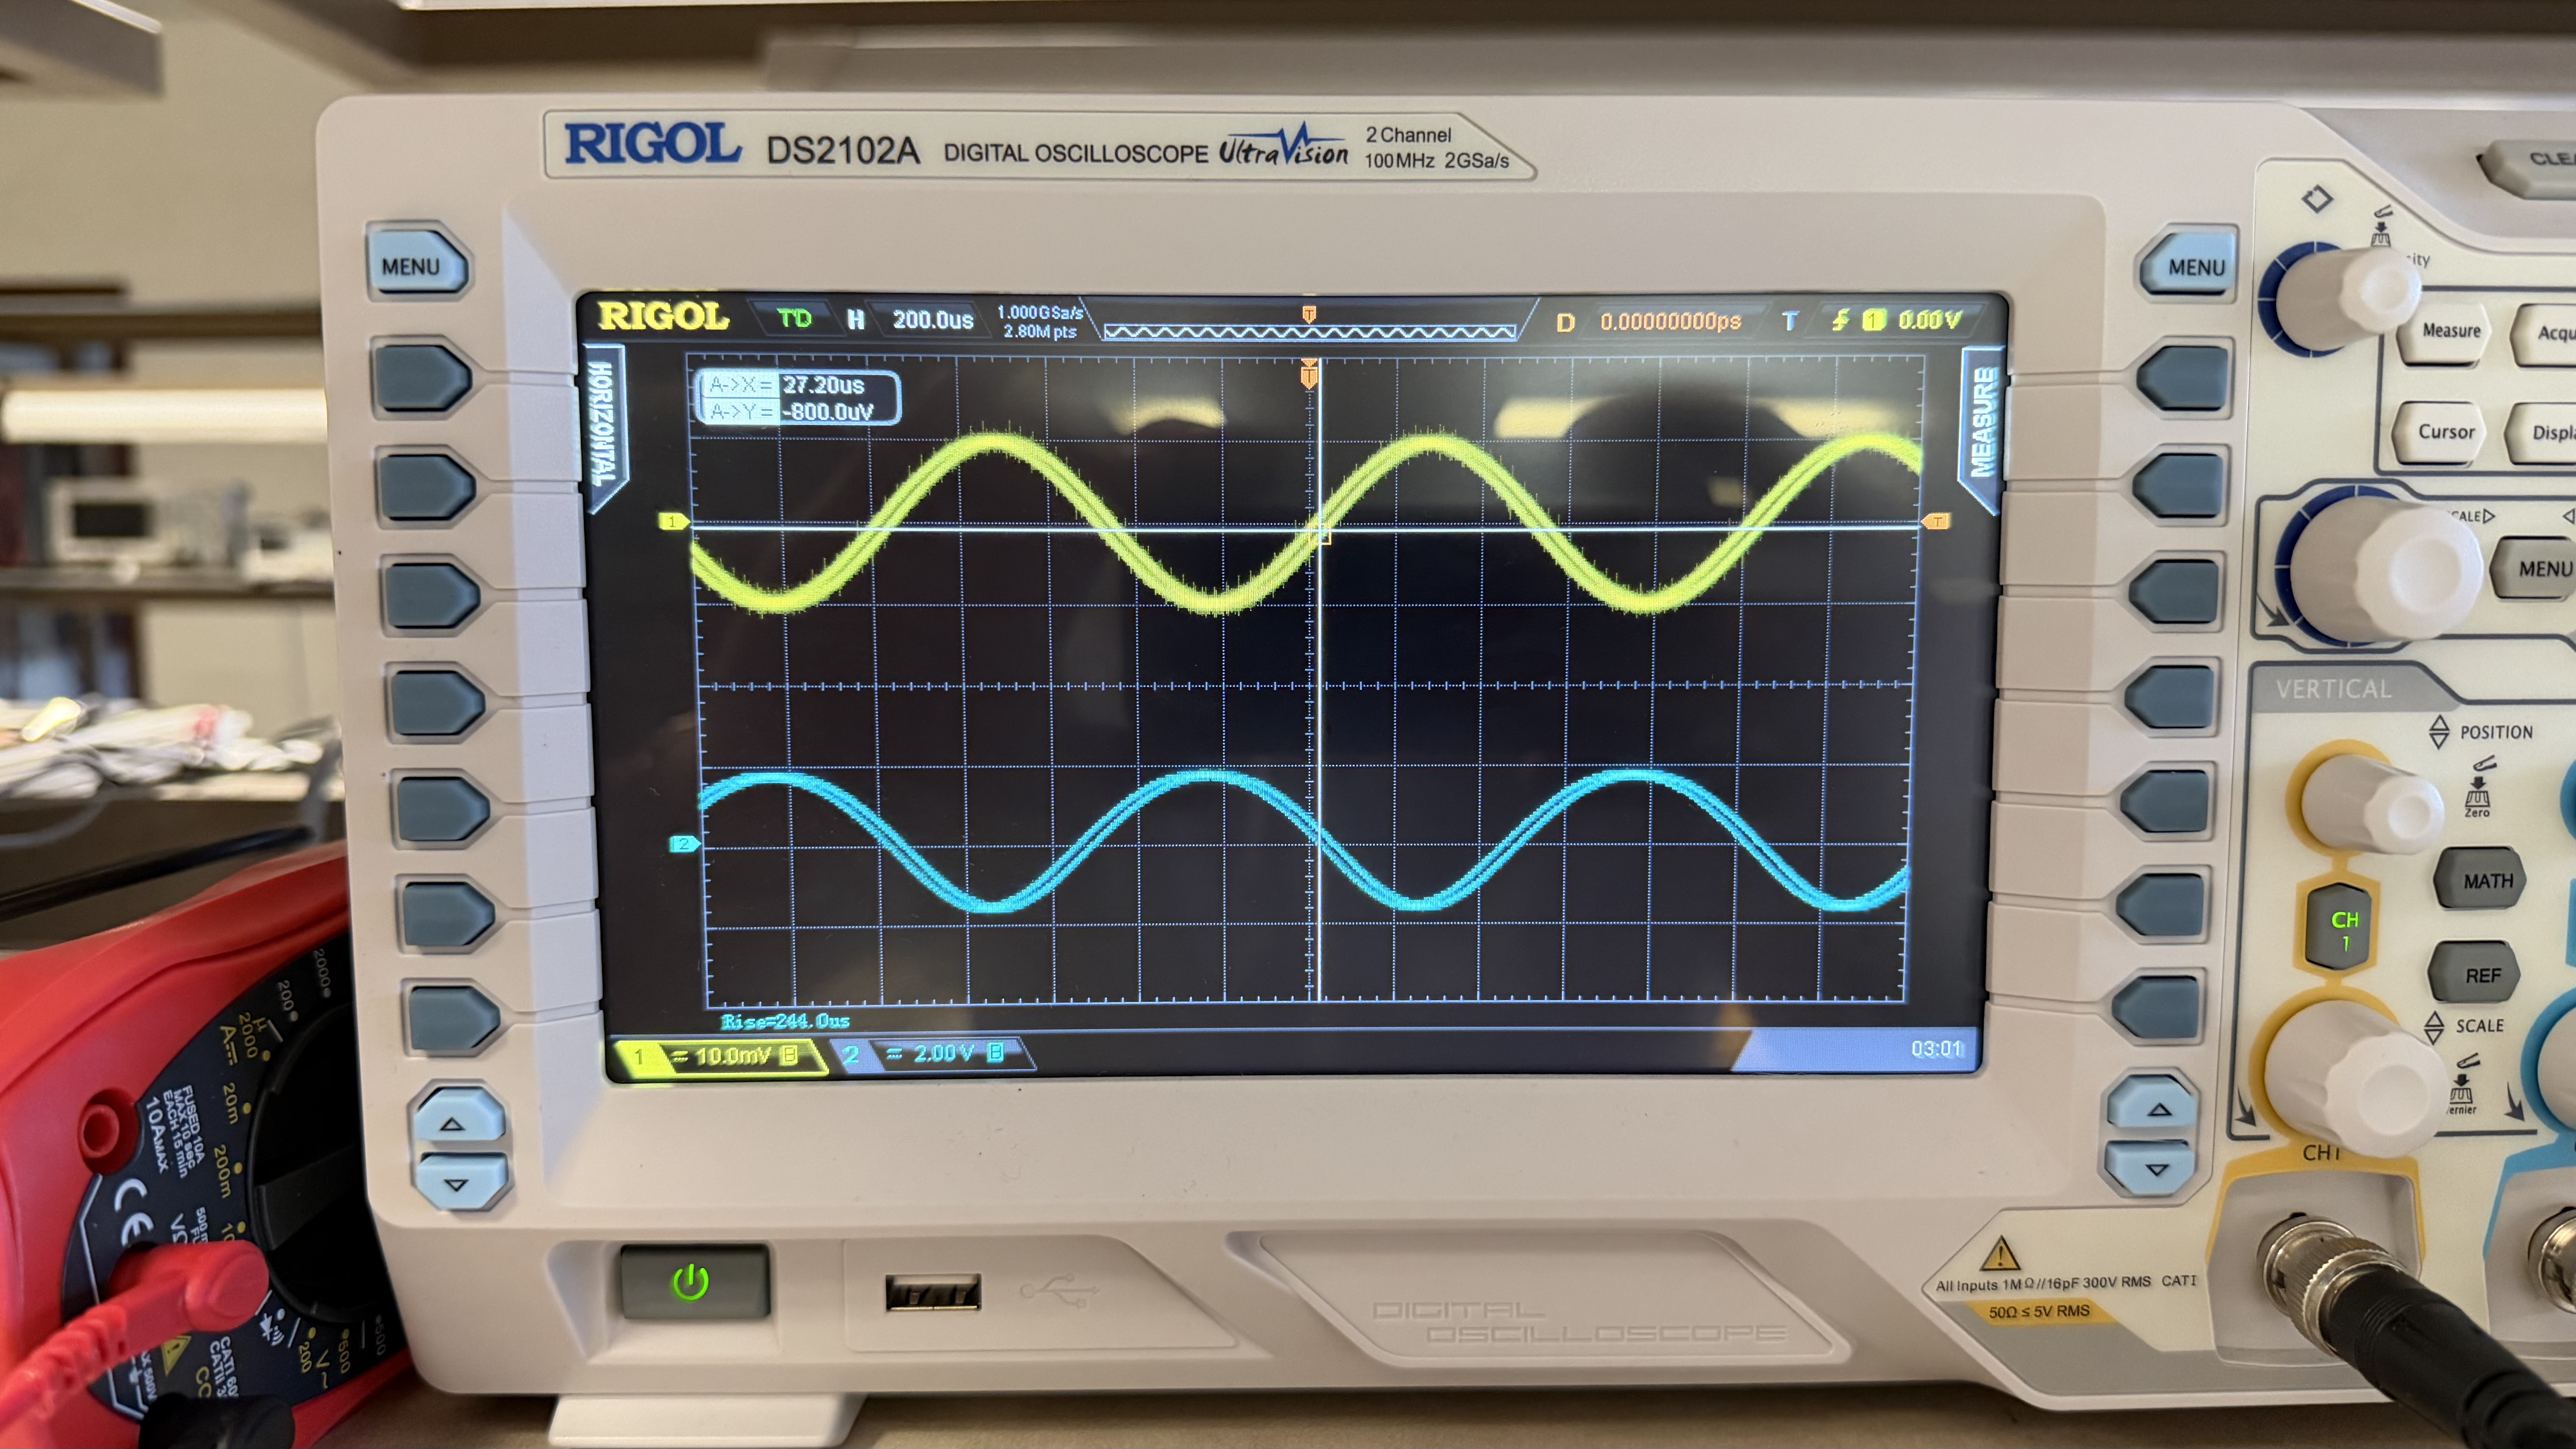
\includegraphics[width=\textwidth]{IMG_0894.png}
        \caption{Loaded ($R_L = \SI{9.1}{k\Omega}$): Output Amplitude drops.}
        \label{fig:loaded}
    \end{subfigure}
    \caption{Determination of Output Resistance. Comparing the output voltage between an open load and a $\SI{9.1}{k\Omega}$ load.}
    \label{fig:ro_meas}
\end{figure}

\textbf{Calculation:}
The output voltage drops significantly when the $\SI{9.1}{k\Omega}$ load is applied compared to the open circuit ($\SI{1}{M\Omega}$) case. Since the voltage drop is roughly 50\%, this indicates that the internal output resistance $R_o$ is approximately equal to the load resistance used:
$$ R_{o} \approx \SI{9.1}{k\Omega} \text{ to } \SI{10}{k\Omega} $$
This matches the theoretical prediction that $R_o \approx R_C = \SI{10.8}{k\Omega}$.

\subsection{Clipping and Distortion}
To test the dynamic range, the input voltage was increased significantly. Figure \ref{fig:clipping} shows the output waveform distorting (clipping) at the bottom rail.

\begin{figure}[H]
    \centering
    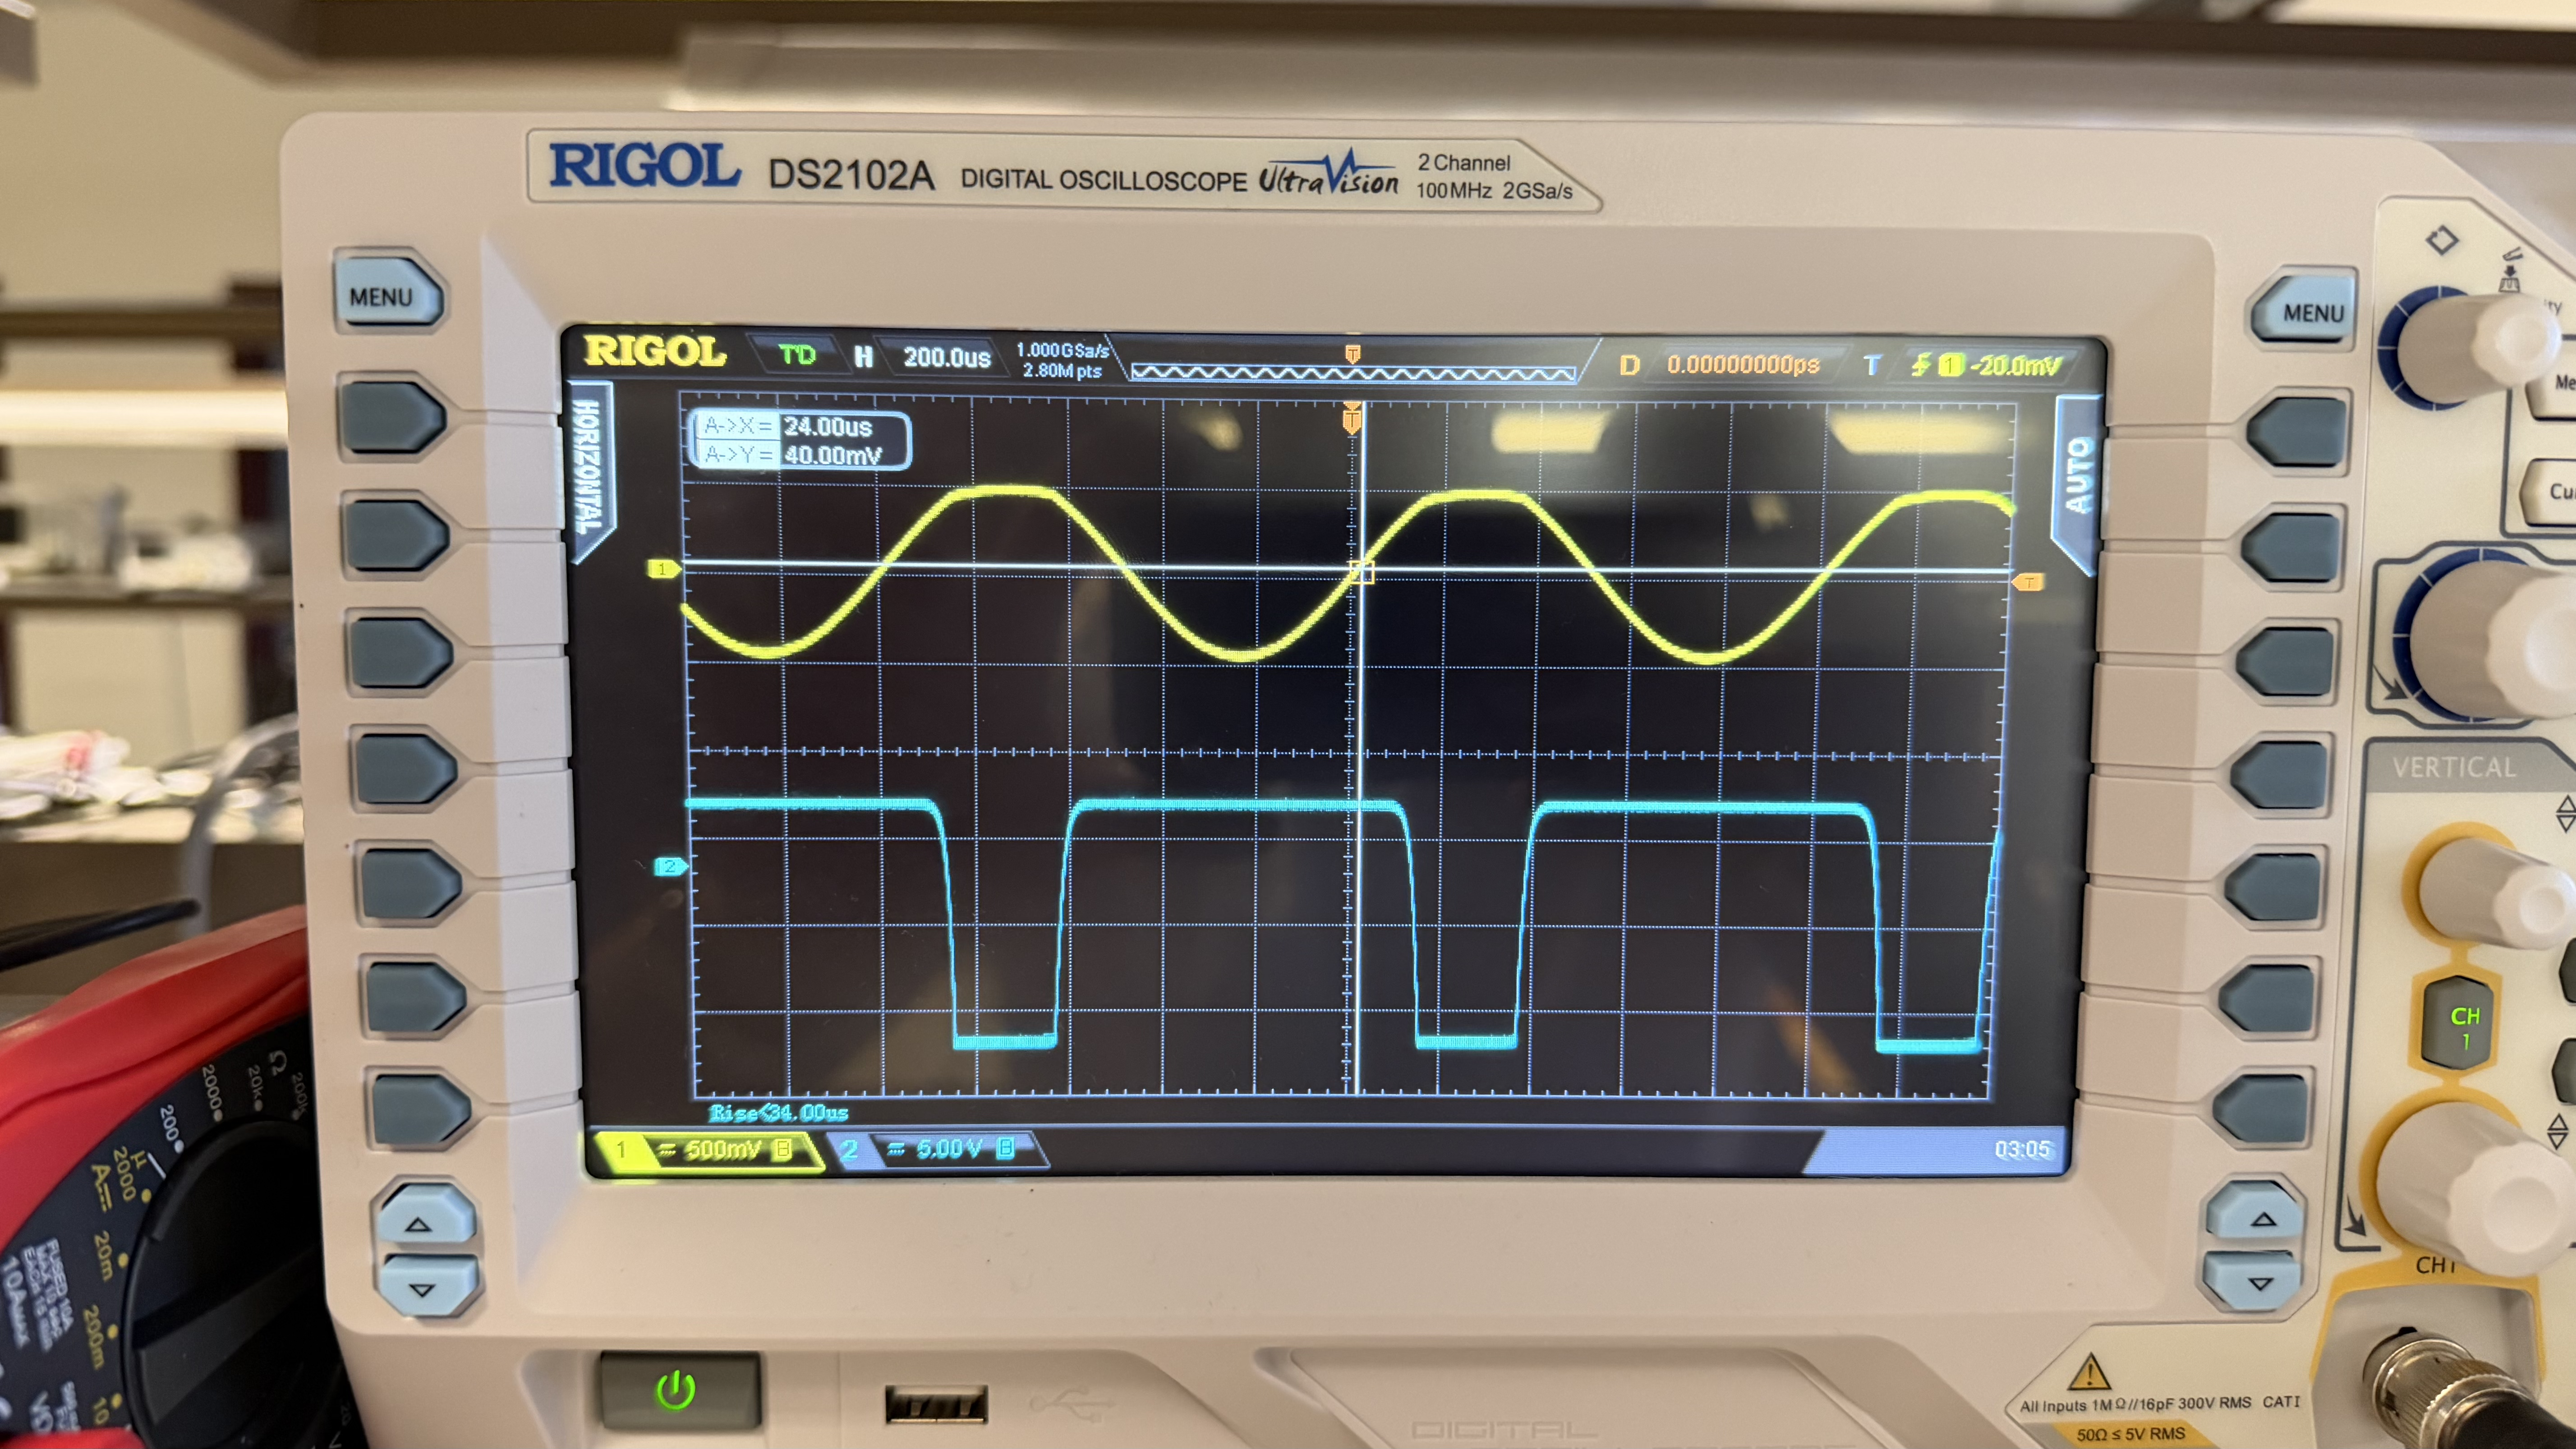
\includegraphics[width=0.7\textwidth]{IMG_0895.png}
    \caption{Output signal showing saturation/clipping when the input amplitude is increased.}
    \label{fig:clipping}
\end{figure}

The clipping occurs because the transistor enters the saturation or cutoff regions when the signal swing exceeds the available headroom defined by the DC operating point and power rails.

\section{Conclusion}
The design of the Common-Emitter amplifier was highly successful. The experimental results matched the design requirements almost perfectly.
\begin{enumerate}
    \item The DC bias point was stable with $I_C = \SI{1.01}{mA}$, matching the $\SI{1}{mA}$ target.
    \item The measured AC gain was $\mathbf{-203 \text{ V/V}}$, which is well within experimental tolerance of the $-200 \text{ V/V}$ goal.
    \item The output resistance was confirmed to be controlled by the collector resistor $R_C$.
\end{enumerate}

% --- BIBLIOGRAPHY ---
\section{Bibliography}
[1] Fixel, Debora. "ENGR 305 - Lab 10: BJT Common-Emitter Amplifier." Trinity College, Hartford, CT, November 2025.
\newline

[2] Jameco Electronics. "2N3904 NPN General Purpose Amplifier." Datasheet, Part no. 38359.

\end{document}